LEGGERE BENE APPUNTI PROF Lezioni 4 e 5
% Questo documento è stato quasi tutto ia generato lel

\subsection*{Radiazione di Corpo Nero} \index{Artefatti pre-qm ! Radiazione di Corpo Nero}
La radiazione di corpo nero è l'emissione elettromagnetica di un oggetto ideale che assorbe perfettamente tutta la radiazione incidente. La distribuzione spettrale di questa radiazione dipende solo dalla temperatura del corpo.

Nel 1900, Lord Rayleigh e James Jeans proposero una formula per descrivere questa radiazione basata sulla fisica classica:

\[
	u(\nu,T) = \frac{8\pi\nu^2}{c^3}k_BT
\]

dove $u(\nu,T)$ è la densità di energia per unità di volume e frequenza, $k_B$ è la costante di Boltzmann, $T$ è la temperatura assoluta, e $\nu$ è la frequenza.

Questa formula, nota come legge di Rayleigh-Jeans, funzionava bene per basse frequenze ma falliva clamorosamente alle alte frequenze, predicendo una energia infinita (la cosiddetta "catastrofe ultravioletta").

\begin{figure}[h]
\centering
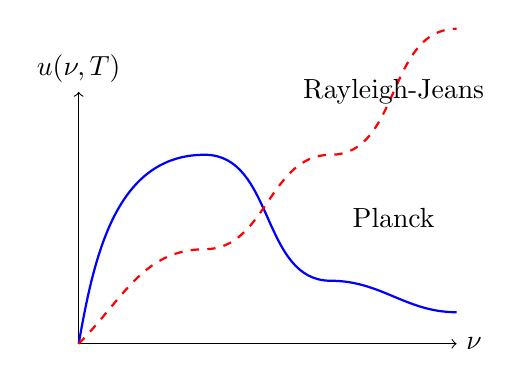
\begin{tikzpicture}[scale=0.8]
	\draw[->] (0,0) -- (6,0) node[right] {$\nu$};
	\draw[->] (0,0) -- (0,4) node[above] {$u(\nu,T)$};
	\draw[thick, blue] (0,0) to[out=80,in=180] (2,3) to[out=0,in=180] (4,1) to[out=0,in=180] (6,0.5);
	\draw[thick, red, dashed] (0,0) to[out=45,in=180] (2,1.5) to[out=0,in=180] (4,3) to[out=0,in=180] (6,5);
	\node at (5,4) {Rayleigh-Jeans};
	\node at (5,2) {Planck};
\end{tikzpicture}
\caption{Confronto tra la legge di Rayleigh-Jeans (tratteggiata) e la legge di Planck}
\end{figure}


Max Planck risolse questo "paradosso" introducendo una ipotesi rivoluzionaria: l'energia può essere emessa o assorbita solo in quantità discrete (quanti) proporzionali alla frequenza:

\[
	E = h\nu
\]

dove $h$ è la costante di Planck. Questo portò alla corretta formula per la radiazione di corpo nero:

\[
	u(\nu,T) = \frac{8\pi h\nu^3}{c^3}\frac{1}{e^{h\nu/k_BT}-1}
\]

\begin{figure}[h]
\centering
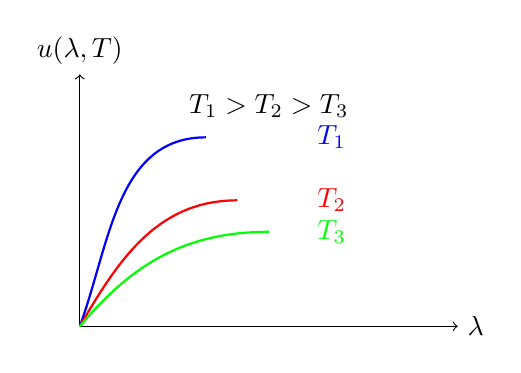
\begin{tikzpicture}[scale=0.8]
	\draw[->] (0,0) -- (6,0) node[right] {$\lambda$};
	\draw[->] (0,0) -- (0,4) node[above] {$u(\lambda,T)$};
	\draw[thick, blue] (0,0) to[out=70,in=180] (2,3);
	\draw[thick, red] (0,0) to[out=60,in=180] (2.5,2);
	\draw[thick, green] (0,0) to[out=50,in=180] (3,1.5);
	\node[blue] at (4,3) {$T_1$};
	\node[red] at (4,2) {$T_2$};
	\node[green] at (4,1.5) {$T_3$};
	\node at (3,3.5) {$T_1 > T_2 > T_3$};
\end{tikzpicture}
\caption{Spettro del corpo nero a diverse temperature}
\end{figure}

Questa nuova visione è stata il primo passo verso la \MQ come oggi è nota.

\subsection*{Effetto Fotoelettrico} \index{Artefatti pre-qm ! Effetto fotoelettrico}
L'effetto fotoelettrico è un fenomeno fisico che consiste nell'emissione di elettroni da parte di un materiale colpito da radiazione elettromagnetica. Questo fenomeno fu osservato per la prima volta da Heinrich Hertz nel 1887.

La teoria classica dell'elettromagnetismo prevedeva che l'energia cinetica degli elettroni emessi dovesse aumentare con l'intensità della radiazione incidente. Tuttavia, gli esperimenti mostrarono che:

\begin{itemize}
	\item L'energia cinetica degli elettroni emessi dipende solo dalla frequenza della radiazione, non dalla sua intensità
	\item Esiste una frequenza di soglia $\nu_0$ al di sotto della quale non si osserva alcuna emissione, indipendentemente dall'intensità
	\item L'emissione degli elettroni è istantanea, senza il ritardo previsto dalla teoria classica
\end{itemize}

Nel 1905, Einstein propose una spiegazione rivoluzionaria basata sulla quantizzazione della luce. Secondo questa teoria, la luce è composta da particelle discrete chiamate fotoni, ciascuno con energia:

\[
	E = h\nu
\]

dove $h$ è la costante di Planck e $\nu$ è la frequenza della radiazione.

Quando un fotone colpisce un elettrone nel materiale, tutta la sua energia viene trasferita. L'energia minima necessaria per estrarre un elettrone dal materiale è detta funzione lavoro $\Phi$. L'energia cinetica dell'elettrone emesso è quindi:

\[
	E_k = h\nu - \Phi
\]

Questa equazione, nota come equazione di Einstein per l'effetto fotoelettrico, spiega perfettamente tutte le osservazioni sperimentali e valse a Einstein il Premio Nobel nel 1921. L'intensità della radiazione determina solo il numero di fotoni e quindi il numero di elettroni emessi, ma non la loro energia.

L'effetto fotoelettrico costituisce una delle prime e più convincenti prove della natura quantistica della luce, dimostrando che in determinate condizioni la radiazione elettromagnetica si comporta come un flusso di particelle discrete anziché come un'onda continua.


\subsection*{Spettri d'emissione}\index{Artefatti pre-qm ! Spettri atomici}
Dalle osservazioni degli spettri d'assorbimento (o d'emissione) risulta che la distrubizione delle frequenze emesse (o assorbite) non è continua, né dipendente dall'intensità, ma è discreta. Risulta che i dati raccolti sono rappresentabili dalla legge:
\[
	\inv \lambda = R \l\inv{n_t^2} + \inv{n^2}\r
\]
In sostanza si osservavano diverse (variando $n_t$) delle 'accumulazioni' di lunghezze d'onda (variando $n$).\\
Questi risultati hanno ispirato il modello atomico \textbf{Planetario di Bohr}, che riporta le proprietà di stazionarietà degli orbitali, e quantizzazione delle energie associate e dei raggi d'orbita. In sostanza esiste un'energia 'minima' che un'interazione fisica può trasformare.

È anche possibile calcolare i raggi di questi 'livelli' (per l'atomo d'idrogeno):
\[
	R_H = \frac{2\pi^2 \mu e^2}{c \h^3}
\]
dove $\mu$ è la massa ridotta ($\sim 1$), e l'energia associata:
\[
E_n = -\frac{m}{2}\frac{e^4}{n^2 \h^2}
\]
% Gli spettri d'emissione discreti osservati negli atomi rappresentano una delle evidenze più dirette della quantizzazione dell'energia nei sistemi microscopici. Storicamente, l'osservazione di righe spettrali ben definite, come quelle dell'idrogeno, ha posto seri problemi alla fisica classica, che prevedeva spettri continui per gli atomi. La spiegazione di questo fenomeno è stata possibile solo con l'avvento della meccanica quantistica.

% Nei modelli atomici classici, come quello di Rutherford, gli elettroni orbitano attorno al nucleo sotto l'azione della forza coulombiana. Tuttavia, secondo l'elettrodinamica classica, un elettrone accelerato dovrebbe emettere radiazione continuamente, perdendo energia e spiraleggiando verso il nucleo. Questo non è ciò che si osserva: gli atomi sono stabili e la radiazione emessa è composta da righe discrete.

% La svolta avviene con il modello di Bohr (1913), che introduce la quantizzazione delle orbite elettroniche. Bohr postulò che l'elettrone può occupare solo certe orbite stazionarie, caratterizzate da un momento angolare quantizzato:

% \[
% 	L_n = n\hbar
% \]

% dove $n$ è un numero intero positivo (numero quantico principale) e $\hbar$ è la costante di Planck ridotta. In queste orbite, l'elettrone non emette radiazione. L'energia associata a ciascun livello è data da:

% \[
% 	E_n = -\frac{m_e e^4}{8\varepsilon_0^2 h^2} \frac{1}{n^2}
% \]

% dove $m_e$ è la massa dell'elettrone, $e$ la carica elementare, $\varepsilon_0$ la permittività del vuoto e $h$ la costante di Planck.

% La radiazione viene emessa (o assorbita) solo quando l'elettrone compie un salto quantico tra due livelli energetici. La frequenza della radiazione emessa è determinata dalla differenza di energia tra i livelli:

% \[
% 	h\nu = E_{n_i} - E_{n_f}
% \]

% dove $n_i$ e $n_f$ sono i numeri quantici iniziale e finale. Questo porta alla formazione di righe spettrali ben definite, ciascuna corrispondente a una transizione specifica.

% La meccanica quantistica fornisce una descrizione più accurata tramite l'equazione di Schrödinger. Per l'atomo di idrogeno, la soluzione dell'equazione di Schrödinger porta a livelli energetici quantizzati identici a quelli previsti da Bohr, ma con una giustificazione teorica più solida. Gli stati elettronici sono descritti da funzioni d'onda $\psi_{n,l,m}$, caratterizzate da numeri quantici principali ($n$), angolari ($l$) e magnetici ($m$).

% La probabilità di una transizione tra due stati è determinata dalla regola d'oro di Fermi e dalle regole di selezione, che impongono vincoli sui cambiamenti dei numeri quantici durante una transizione. Ad esempio, per le transizioni dipolari elettriche, il numero quantico angolare deve cambiare di $\Delta l = \pm 1$.

% Ogni elemento chimico ha una struttura elettronica unica, determinata dalla configurazione degli elettroni nei vari livelli quantici. Quando un atomo viene eccitato (ad esempio tramite collisioni o assorbimento di fotoni), uno o più elettroni possono essere promossi a livelli energetici superiori. Il ritorno agli stati fondamentali avviene tramite salti quantici, con emissione di fotoni di energia ben definita. Questo processo genera lo spettro d'emissione caratteristico dell'elemento.

% Nel caso dell'idrogeno, le transizioni tra livelli energetici danno origine alle serie spettrali (Balmer, Lyman, Paschen, ecc.), ciascuna corrispondente a transizioni verso uno specifico livello finale. Ad esempio, la serie di Balmer corrisponde a transizioni verso $n_f = 2$ e produce righe visibili.

% Negli atomi polielettronici, la struttura degli spettri è più complessa a causa delle interazioni tra elettroni (effetti di schermatura, accoppiamento spin-orbita, ecc.), ma il principio di base rimane invariato: solo certe transizioni sono permesse e ciascuna corrisponde a una riga spettrale.

% La discrezione degli spettri d'emissione è dunque una conseguenza diretta della quantizzazione dei livelli energetici negli atomi e della natura quantistica delle transizioni elettroniche. Ogni salto quantico produce un fotone di energia ben definita, osservabile come una riga nello spettro. Questo fenomeno è alla base di molte tecniche spettroscopiche e ha permesso di identificare la composizione chimica di stelle e galassie, oltre a fornire una conferma sperimentale fondamentale della meccanica quantistica.

% In sintesi, gli spettri d'emissione discreti sono il risultato dei salti quantici degli elettroni tra livelli energetici quantizzati. La posizione e l'intensità delle righe spettrali dipendono dalla struttura elettronica dell'atomo e dalle regole di selezione imposte dalla meccanica quantistica. Questo quadro teorico spiega in modo completo le osservazioni sperimentali e costituisce uno dei pilastri della fisica moderna.


\subsection*{Effetto Isotopico}\index{Artefatti pre-qm ! Effetto isotropico}
Se si osserva lo spettro d'emissione di una miscela di idrogeno a base di deuterio e trizio, risulta che le linee spetrali seguono sì la legge appena definita, ma invece di vedere delle linee singole si osservavano linee accoppiate invece che isolate. Questo fatto è una diretta conseguenza dei calcoli appena fatti: risulta infatti che la massa ridotta dell trizio differisce di una parte su 4'000 da quella del deuterio, e quindi, per il principio di sovrapposizione, i due isotopi sono da considerarsi gas diversi, quindi con due diversi spettri d'emissione.

\subsection*{Principio di Corrispondenza}\index{Artefatti pre-qm ! Principio di corrispondenza}
Ora rimane solo la verifica che questi nuovi principi appena introdotti siano in accordo anche con le misurazioni classiche: è necessario che su larga scala le previsioni della meccanica quantistica risulti in accordo con le misurazioni classiche.\\
Il problema si pone quando si hanno energie molto più grandi della scala delle energie di legame. Vediamo qual'è la differenza d'energia di due livelli adiacenti con $n$ molto grande, partendo dall'energia di un'onda elettromagnetica:
\[
	E_n - E_{n-1} = \h \l\nu_{n \rightarrow n-1}\r = -R\h c\sim \frac{2R\h c}{n^3}
\]
da cui si può derivare anche che la frequenza del fotono emesso nella transizione è:
\[
	\nu_{n \rightarrow n+1}^2 \sim \frac{2|E_n|^3}{\pi^2 m e^4}
\]
che tra l'altro coincide con la frequenza di rivoluzione dell'orbita dell'elettrone.\\
Questi risultati suggeriscono che, per $n$ molto grandi, l'energia del salto di livello diventa trascurabile, e la frequenza dei fotoni emessi rimane pressoché costante \\\\

Da evidenziare il fatto che l'unità di misura di $\h$ è $J\cdots$, Joule per secondo.